\section{Alerting and Profiling}

\begin{frame}{Real-Time Alert Engine (\texttt{src/alerts.py})}
    \begin{itemize}
        \setlength{\itemsep}{11pt}
        \item \textbf{What It Is:} A lightweight tool that monitors system health (CPU, RAM, temperatures) and notifies you when safety limits are exceeded.
        \item \textbf{How It Works:} Only alerts if high load lasts for several readings in a row (ignoring brief spikes), uses cooldowns to avoid spam, and auto-resolves when levels return to normal.
        \item \textbf{Topics Covered:}
        \begin{itemize}
            \setlength{\itemsep}{4pt}
            \item \textbf{Finding the Culprit:} Identifies which app or process is causing the spike.
            \item \textbf{Smart Data Handling:} Ignores cleaner gap-fills to prevent false alarms.
            \item \textbf{Alert Channels:} Sends desktop popups and updates the web dashboard in real time.
        \end{itemize}
    \end{itemize}
\end{frame}

\begin{frame}{Performance Profiling and Hardware Optimizations}
    \begin{itemize}
        \setlength{\itemsep}{4pt}
        \item \textbf{Minimal Probe Footprint:} Collector CPU is under \textbf{0.74\%} even under stress load, using just \textbf{4.2 MB} RAM.
        \item \textbf{Eliminated GPU Wakeup Stalls:} Skips \texttt{nvidia-smi} when dGPU sleeps in D3cold, slashing latency from \textbf{520 ms to 34 ms}.
        \item \textbf{Smart Pipeline Caching:} Stamp caching and \texttt{--since} filtering make analysis up to \textbf{6.2$\times$ faster}.
    \end{itemize}
    \vspace{0.3em}
    \centering
    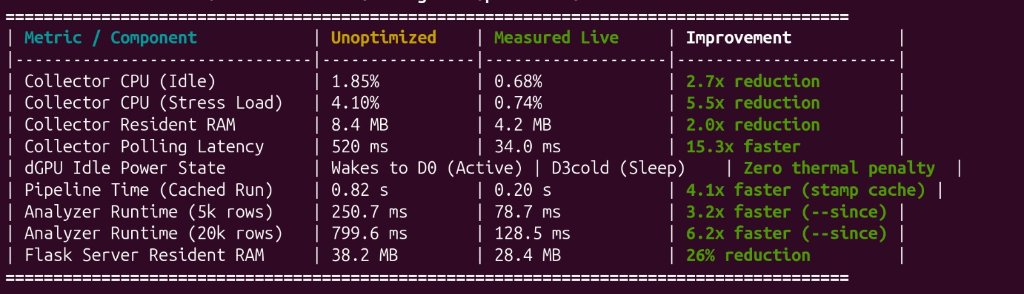
\includegraphics[width=0.92\textwidth]{figures/profiling_benchmarks.jpg}
\end{frame}
